% Options for packages loaded elsewhere
\PassOptionsToPackage{unicode}{hyperref}
\PassOptionsToPackage{hyphens}{url}
\PassOptionsToPackage{dvipsnames,svgnames,x11names}{xcolor}
\documentclass[
  10pt,
]{extarticle}
\usepackage{xcolor}
\usepackage[top=1.5in, bottom=1.5in, left=1.5in, right=1.5in]{geometry}
\usepackage{amsmath,amssymb}
\setcounter{secnumdepth}{5}
\usepackage{iftex}
\ifPDFTeX
  \usepackage[T1]{fontenc}
  \usepackage[utf8]{inputenc}
  \usepackage{textcomp} % provide euro and other symbols
\else % if luatex or xetex
  \usepackage{unicode-math} % this also loads fontspec
  \defaultfontfeatures{Scale=MatchLowercase}
  \defaultfontfeatures[\rmfamily]{Ligatures=TeX,Scale=1}
\fi
\usepackage{lmodern}
\ifPDFTeX\else
  % xetex/luatex font selection
\fi
% Use upquote if available, for straight quotes in verbatim environments
\IfFileExists{upquote.sty}{\usepackage{upquote}}{}
\IfFileExists{microtype.sty}{% use microtype if available
  \usepackage[]{microtype}
  \UseMicrotypeSet[protrusion]{basicmath} % disable protrusion for tt fonts
}{}
\makeatletter
\@ifundefined{KOMAClassName}{% if non-KOMA class
  \IfFileExists{parskip.sty}{%
    \usepackage{parskip}
  }{% else
    \setlength{\parindent}{0pt}
    \setlength{\parskip}{6pt plus 2pt minus 1pt}}
}{% if KOMA class
  \KOMAoptions{parskip=half}}
\makeatother
\usepackage{color}
\usepackage{fancyvrb}
\newcommand{\VerbBar}{|}
\newcommand{\VERB}{\Verb[commandchars=\\\{\}]}
\DefineVerbatimEnvironment{Highlighting}{Verbatim}{commandchars=\\\{\}}
% Add ',fontsize=\small' for more characters per line
\usepackage{framed}
\definecolor{shadecolor}{RGB}{248,248,248}
\newenvironment{Shaded}{\begin{snugshade}}{\end{snugshade}}
\newcommand{\AlertTok}[1]{\textcolor[rgb]{0.94,0.16,0.16}{#1}}
\newcommand{\AnnotationTok}[1]{\textcolor[rgb]{0.56,0.35,0.01}{\textbf{\textit{#1}}}}
\newcommand{\AttributeTok}[1]{\textcolor[rgb]{0.13,0.29,0.53}{#1}}
\newcommand{\BaseNTok}[1]{\textcolor[rgb]{0.00,0.00,0.81}{#1}}
\newcommand{\BuiltInTok}[1]{#1}
\newcommand{\CharTok}[1]{\textcolor[rgb]{0.31,0.60,0.02}{#1}}
\newcommand{\CommentTok}[1]{\textcolor[rgb]{0.56,0.35,0.01}{\textit{#1}}}
\newcommand{\CommentVarTok}[1]{\textcolor[rgb]{0.56,0.35,0.01}{\textbf{\textit{#1}}}}
\newcommand{\ConstantTok}[1]{\textcolor[rgb]{0.56,0.35,0.01}{#1}}
\newcommand{\ControlFlowTok}[1]{\textcolor[rgb]{0.13,0.29,0.53}{\textbf{#1}}}
\newcommand{\DataTypeTok}[1]{\textcolor[rgb]{0.13,0.29,0.53}{#1}}
\newcommand{\DecValTok}[1]{\textcolor[rgb]{0.00,0.00,0.81}{#1}}
\newcommand{\DocumentationTok}[1]{\textcolor[rgb]{0.56,0.35,0.01}{\textbf{\textit{#1}}}}
\newcommand{\ErrorTok}[1]{\textcolor[rgb]{0.64,0.00,0.00}{\textbf{#1}}}
\newcommand{\ExtensionTok}[1]{#1}
\newcommand{\FloatTok}[1]{\textcolor[rgb]{0.00,0.00,0.81}{#1}}
\newcommand{\FunctionTok}[1]{\textcolor[rgb]{0.13,0.29,0.53}{\textbf{#1}}}
\newcommand{\ImportTok}[1]{#1}
\newcommand{\InformationTok}[1]{\textcolor[rgb]{0.56,0.35,0.01}{\textbf{\textit{#1}}}}
\newcommand{\KeywordTok}[1]{\textcolor[rgb]{0.13,0.29,0.53}{\textbf{#1}}}
\newcommand{\NormalTok}[1]{#1}
\newcommand{\OperatorTok}[1]{\textcolor[rgb]{0.81,0.36,0.00}{\textbf{#1}}}
\newcommand{\OtherTok}[1]{\textcolor[rgb]{0.56,0.35,0.01}{#1}}
\newcommand{\PreprocessorTok}[1]{\textcolor[rgb]{0.56,0.35,0.01}{\textit{#1}}}
\newcommand{\RegionMarkerTok}[1]{#1}
\newcommand{\SpecialCharTok}[1]{\textcolor[rgb]{0.81,0.36,0.00}{\textbf{#1}}}
\newcommand{\SpecialStringTok}[1]{\textcolor[rgb]{0.31,0.60,0.02}{#1}}
\newcommand{\StringTok}[1]{\textcolor[rgb]{0.31,0.60,0.02}{#1}}
\newcommand{\VariableTok}[1]{\textcolor[rgb]{0.00,0.00,0.00}{#1}}
\newcommand{\VerbatimStringTok}[1]{\textcolor[rgb]{0.31,0.60,0.02}{#1}}
\newcommand{\WarningTok}[1]{\textcolor[rgb]{0.56,0.35,0.01}{\textbf{\textit{#1}}}}
\usepackage{longtable,booktabs,array}
\usepackage{calc} % for calculating minipage widths
% Correct order of tables after \paragraph or \subparagraph
\usepackage{etoolbox}
\makeatletter
\patchcmd\longtable{\par}{\if@noskipsec\mbox{}\fi\par}{}{}
\makeatother
% Allow footnotes in longtable head/foot
\IfFileExists{footnotehyper.sty}{\usepackage{footnotehyper}}{\usepackage{footnote}}
\makesavenoteenv{longtable}
\usepackage{graphicx}
\makeatletter
\newsavebox\pandoc@box
\newcommand*\pandocbounded[1]{% scales image to fit in text height/width
  \sbox\pandoc@box{#1}%
  \Gscale@div\@tempa{\textheight}{\dimexpr\ht\pandoc@box+\dp\pandoc@box\relax}%
  \Gscale@div\@tempb{\linewidth}{\wd\pandoc@box}%
  \ifdim\@tempb\p@<\@tempa\p@\let\@tempa\@tempb\fi% select the smaller of both
  \ifdim\@tempa\p@<\p@\scalebox{\@tempa}{\usebox\pandoc@box}%
  \else\usebox{\pandoc@box}%
  \fi%
}
% Set default figure placement to htbp
\def\fps@figure{htbp}
\makeatother
\setlength{\emergencystretch}{3em} % prevent overfull lines
\providecommand{\tightlist}{%
  \setlength{\itemsep}{0pt}\setlength{\parskip}{0pt}}
\usepackage{xcolor}
\usepackage{hyperref}
\hypersetup{colorlinks=true, linkcolor=blue, urlcolor=blue, citecolor=blue}
\usepackage{float}
\usepackage{fvextra}
\usepackage{fancyhdr}
\usepackage{lastpage}
\usepackage{soul}
\usepackage{etoolbox}
\usepackage{microtype}
\usepackage{tcolorbox}
\usepackage{enumitem}
\usepackage{fancyvrb}
\usepackage{xspace}
\allowdisplaybreaks
\setcounter{tocdepth}{2}
\setcounter{secnumdepth}{0}
\floatplacement{figure}{H}
\makeatletter
\newcommand{\@subtitle}{}
\newcommand{\subtitle}[1]{\gdef\@subtitle{#1}}
\newcommand{\DocSubtitle}{\@subtitle}
\renewcommand{\maketitle}{
  \thispagestyle{plain}
  \null
  \vfill
  \begin{center}
    {\Large \textsc{\@title} \par}\vskip 0.5em
    {\LARGE \bfseries \@subtitle \par}\vskip 0.75em
    {\large \@author \par}\vskip 0.5em
    {\normalsize \@date \par}
  \end{center}
  \vfill
  \tableofcontents
  \vspace{1em}
  \clearpage
}
\AfterEndEnvironment{Highlighting}{\setcounter{CodeLine}{\numexpr\value{CodeLine}+\FV@CodeLineNo\relax}}
\makeatother
\fancypagestyle{plain}{
  \fancyhf{}
  \renewcommand{\headrulewidth}{0pt}
  \renewcommand{\footrulewidth}{0pt}
}
\pagestyle{fancy}
\fancyhf{}
\fancyfoot[C]{\small\textsc{Page}~\thepage~\textsc{of}~\pageref{LastPage}}
\fancyhead[L]{\textsc{Rento Saijo}}
\fancyhead[R]{\textsc{\DocSubtitle}}
\fancyhead[C]{\textsc{\rightmark}}
\renewcommand{\headrulewidth}{0.5pt}
\renewcommand{\footrulewidth}{0.5pt}
\newcounter{CodeLine}
\newcounter{cell}
\AtBeginEnvironment{Highlighting}{\stepcounter{cell}}
\DefineVerbatimEnvironment{Highlighting}{Verbatim}{
  frame=single,
  rulecolor=\color{black},
  framesep=2mm,
  label=\footnotesize Cell \thecell,
  labelposition=topline,
  commandchars=\\\{\},
  breaklines=true,
  breakanywhere=false,
  breaksymbol={},
  numbers=left,
  numbersep=3pt,
  firstnumber=\numexpr\value{CodeLine}+1\relax,
  fontsize=\small
}
\DefineVerbatimEnvironment{verbatim}{Verbatim}{
  breaklines=true,
  breakanywhere=true,
  numbers=left,
  numbersep=3pt,
  firstnumber=1,
  fontsize=\footnotesize
}
\newtcolorbox{problem}[1][]{
  title={\textsc{#1}}
}
\newenvironment{alphenum}{
  \begin{enumerate}[
    label=(\alph*),
    itemsep=3pt,
    parsep=0pt,
    topsep=6pt
  ]
}{
  \end{enumerate}
}
\newenvironment{items}{
  \begin{itemize}[
    itemsep=3pt,
    parsep=0pt,
    topsep=6pt
  ]
}{
  \end{itemize}
}
\renewcommand{\contentsname}{Table of Contents}
\newcommand{\E}{\mathrm{E}}
\newcommand{\Var}{\mathrm{Var}}
\newcommand{\R}{\textsf{R}\xspace}
\newcommand{\SD}{\mathrm{SD}}
\newcommand{\SE}{\mathrm{SE}}
\usepackage{bookmark}
\IfFileExists{xurl.sty}{\usepackage{xurl}}{} % add URL line breaks if available
\urlstyle{same}
\hypersetup{
  pdftitle={STA 209: Introduction to Time Series Analysis},
  colorlinks=true,
  linkcolor={blue},
  filecolor={Maroon},
  citecolor={blue},
  urlcolor={blue},
  pdfcreator={LaTeX via pandoc}}

\title{STA 209: Introduction to Time Series Analysis}
\usepackage{etoolbox}
\makeatletter
\providecommand{\subtitle}[1]{% add subtitle to \maketitle
  \apptocmd{\@title}{\par {\large #1 \par}}{}{}
}
\makeatother
\subtitle{Homework 3}
\author{Rento Saijo}
\date{March 4, 2026}

\begin{document}
\maketitle

\section{Disclosure}\label{disclosure}

GPT-5.3-Codex was used to create the \texttt{YAML} portion and some \texttt{LaTeX} code to format the text/equations nicely. Page formatting code was also provided by Derin Gezgin. In the setup chunk, libraries were loaded and some helper functions were defined including but not limited to \texttt{table\_latex()} and \texttt{seasonal\_df()}. See the original \texttt{RMD} file \href{https://github.com/RentoSaijo/STA209/blob/main/Homework3.Rmd}{here} for more details.

\newpage

\section{Problem 1}\label{problem-1}

\begin{problem}[Problem 1]
From \texttt{astsa} package consider the weekly time series \texttt{oil} and \texttt{gas}. The oil series is in dollars per barrel while the gas series is in cents per gallon. In the package \texttt{astsa}, see \texttt{?oil} and \texttt{?gas} for explanation. These data have 545 weekly values from 2000 to mid 2010.
\end{problem}

\begin{Shaded}
\begin{Highlighting}[]
\CommentTok{\# Load data.}
\FunctionTok{library}\NormalTok{(astsa)}
\FunctionTok{data}\NormalTok{(oil)}
\FunctionTok{data}\NormalTok{(gas)}
\CommentTok{\#?oil}
\CommentTok{\#?gas}
\end{Highlighting}
\end{Shaded}

\begin{itemize}
\tightlist
\item
  \texttt{oil}: Crude oil; WTI spot price FOB (in dollars/barrel); weekly from 2000 to mid-2010.
\item
  \texttt{gas}: New York Harbor conventional regular gasoline weekly spot price FOB (in cents/gallon) from 2000 to mid-2010.
\end{itemize}

\newpage

\subsection{Problem 1 (a)}\label{problem-1-a}

\begin{problem}[Problem 1 (a)]
Plot the two series on the same graph. Comment on the characteristics.
\end{problem}

\begin{Shaded}
\begin{Highlighting}[]
\CommentTok{\# Plot time series.}
\FunctionTok{tsplot}\NormalTok{(}
  \FunctionTok{cbind}\NormalTok{(}\StringTok{\textasciigrave{}}\AttributeTok{Oil (Dollars/Barrel)}\StringTok{\textasciigrave{}} \OtherTok{=}\NormalTok{ oil, }\StringTok{\textasciigrave{}}\AttributeTok{Gas (Cents/Gallon)}\StringTok{\textasciigrave{}} \OtherTok{=}\NormalTok{ gas),}
  \AttributeTok{spaghetti =} \ConstantTok{TRUE}\NormalTok{,}
  \AttributeTok{addLegend =} \ConstantTok{TRUE}\NormalTok{,}
  \AttributeTok{location =} \StringTok{\textquotesingle{}topleft\textquotesingle{}}\NormalTok{,}
  \AttributeTok{llwd =} \DecValTok{4}\NormalTok{,}
  \AttributeTok{col  =} \FunctionTok{c}\NormalTok{(}\StringTok{\textquotesingle{}firebrick\textquotesingle{}}\NormalTok{, }\StringTok{\textquotesingle{}navy\textquotesingle{}}\NormalTok{),}
  \AttributeTok{main =} \StringTok{\textquotesingle{}Weekly Oil and Gas Prices\textquotesingle{}}\NormalTok{,}
  \AttributeTok{xlab =} \StringTok{\textquotesingle{}Time (Weekly Observations)\textquotesingle{}}\NormalTok{,}
  \AttributeTok{ylab =} \StringTok{\textquotesingle{}Price\textquotesingle{}}
\NormalTok{)}
\end{Highlighting}
\end{Shaded}

\begin{center}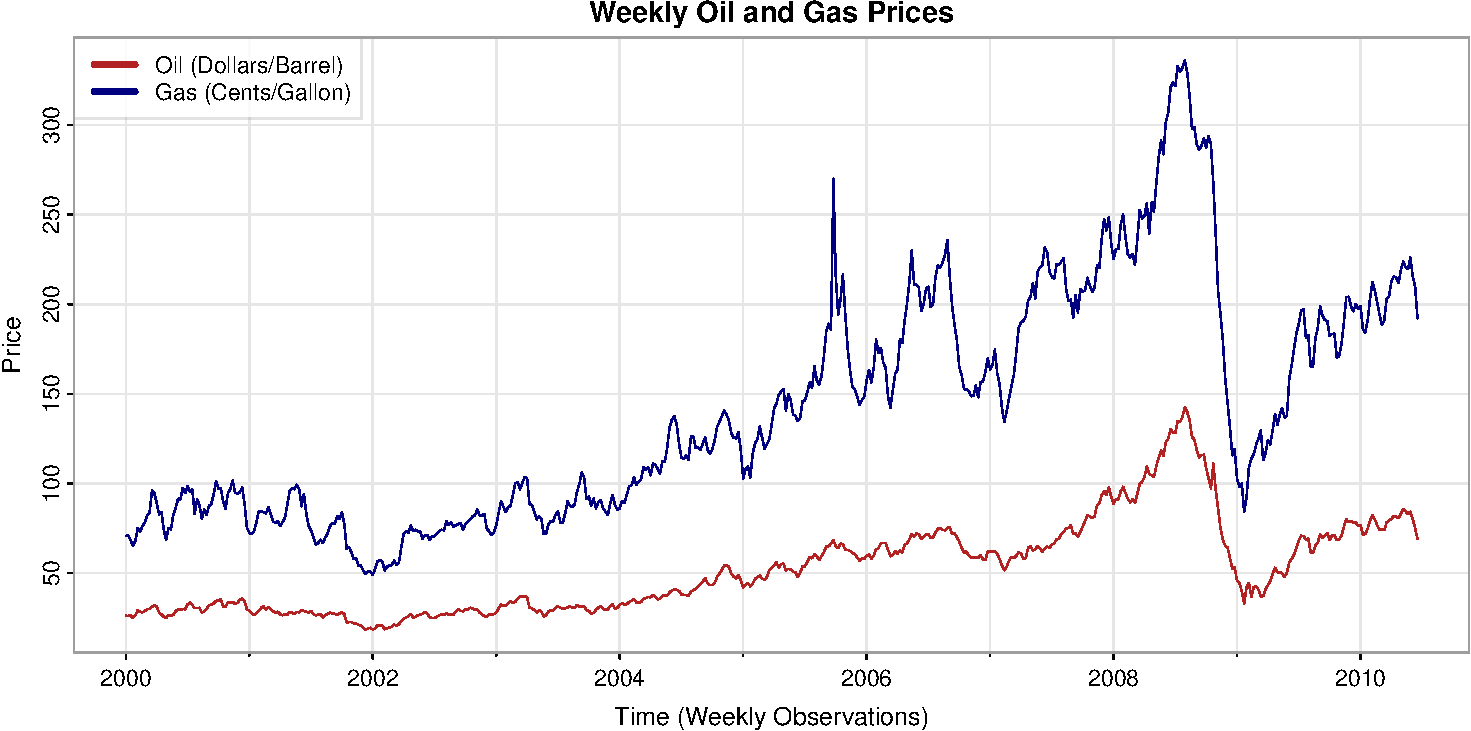
\includegraphics[width=\linewidth]{Homework3_files/figure-latex/unnamed-chunk-3-1} \end{center}

The oil data is weekly crude oil price measured in USD per barrel, and the gas data is weekly gasoline price measured in cents per gallon. Both series have 545 observations from 2000 week 1 to 2010 week 25 with \(frequency=52\). The mean behavior is clearly time-dependent for both series, with an overall upward movement that is non-linear because of the strong rise through 2008, sharp decline, and partial recovery for both oil and gas price. There is no clear repeated seasonal pattern by week-of-year in these series, at least as they are presented currently. The variability is substantial, with oil range \(=124.24\) dollars/barrel and gas range \(=287.12\) cents/gallon, and the variance seems to be be getting gradually larger, so we'd say both series are heteroscedastic. There's a huge crash around 2008-2009 (presumably part of the 2008 financial crisis), so they are both volatile (which already implies that both series are heteroscedastic).

\newpage

\subsection{Problem 1 (b)}\label{problem-1-b}

\begin{problem}[Problem 1 (b)]
In economics, it is often the percentage change in price (returns or growth rate), rather than the absolute price change, that is important. Transform the data as described as \texttt{poil = diff(log(oil))} and \texttt{pgas = diff(log(gas))}. Plot the transformed series in the same plot (\texttt{poil} and \texttt{pgas} on one graph) and comment on the main characteristics of these series.
\end{problem}

\begin{Shaded}
\begin{Highlighting}[]
\CommentTok{\# Plot growth rates.}
\NormalTok{poil }\OtherTok{\textless{}{-}} \FunctionTok{diff}\NormalTok{(}\FunctionTok{log}\NormalTok{(oil)); pgas }\OtherTok{\textless{}{-}} \FunctionTok{diff}\NormalTok{(}\FunctionTok{log}\NormalTok{(gas))}
\FunctionTok{tsplot}\NormalTok{(}
  \FunctionTok{cbind}\NormalTok{(poil, pgas),}
  \AttributeTok{spaghetti =} \ConstantTok{TRUE}\NormalTok{, }\AttributeTok{addLegend =} \ConstantTok{TRUE}\NormalTok{,}
  \AttributeTok{llwd =} \DecValTok{4}\NormalTok{, }\AttributeTok{col  =} \FunctionTok{c}\NormalTok{(}\StringTok{\textquotesingle{}firebrick\textquotesingle{}}\NormalTok{, }\StringTok{\textquotesingle{}navy\textquotesingle{}}\NormalTok{),}
  \AttributeTok{main =} \StringTok{\textquotesingle{}Weekly Oil and Gas Growth Rates (Log Differences)\textquotesingle{}}\NormalTok{,}
  \AttributeTok{xlab =} \StringTok{\textquotesingle{}Time (Weekly Observations)\textquotesingle{}}\NormalTok{,}
  \AttributeTok{ylab =} \StringTok{\textquotesingle{}Weekly Log Growth Rate (Approx. Weekly Percent Change)\textquotesingle{}}
\NormalTok{)}
\end{Highlighting}
\end{Shaded}

\begin{center}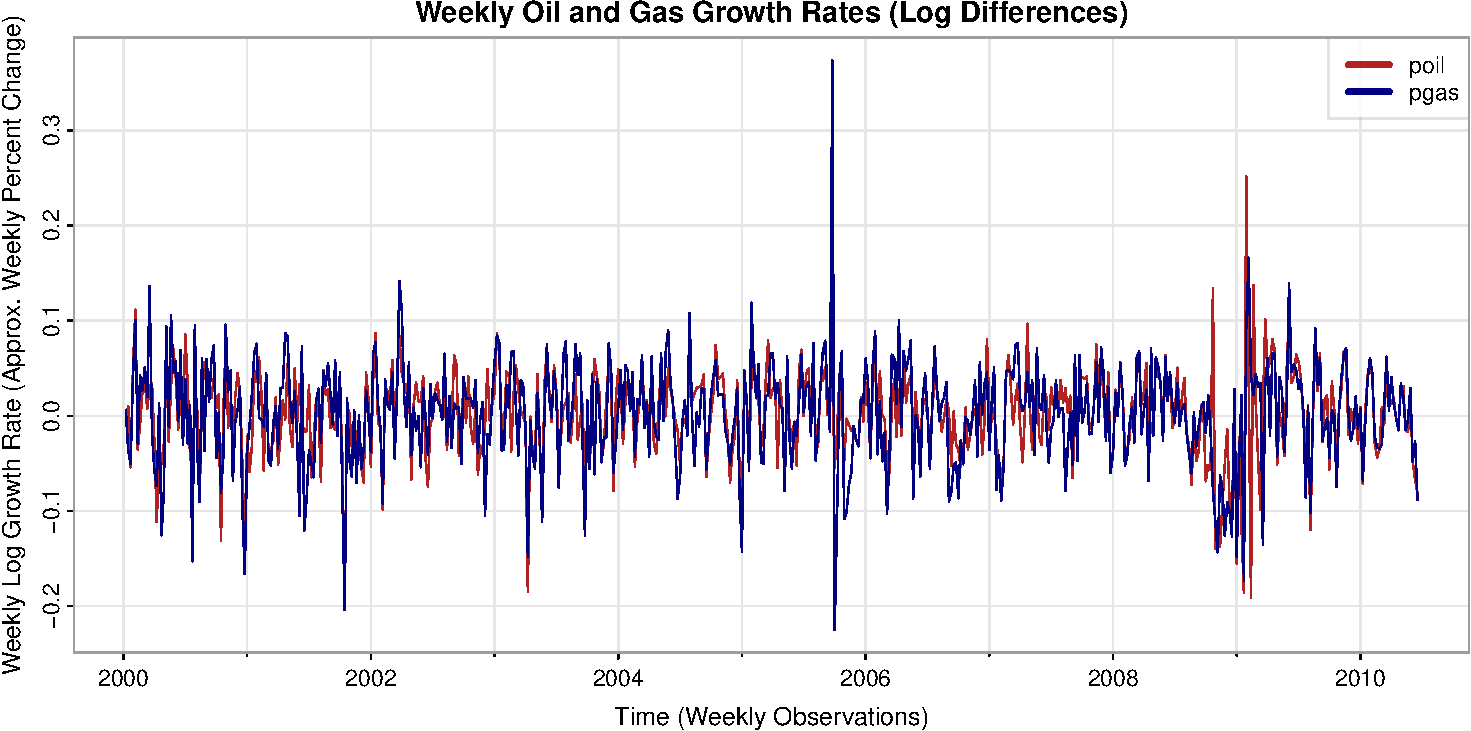
\includegraphics[width=\linewidth]{Homework3_files/figure-latex/unnamed-chunk-4-1} \end{center}

The transformed oil series is \(O_t=\Delta\log(\texttt{oil}_t)\) and the transformed gas series is \(G_t=\Delta\log(\texttt{gas}_t)\), so both are weekly growth rates (approximately weekly percent changes). Each transformed series has 544 observations from 2000 week 2 to 2010 week 25. After transformation, both series are centered near zero (\(\bar O_t=0.00178\), \(\bar G_t=0.00184\)), so no clear deterministic trend remains. There is also no clear repeated seasonal pattern (again, at least with how it's currently presented). The ranges are \(\max(O_t)-\min(O_t)=0.444\) and \(\max(G_t)-\min(G_t)=0.598\), and the variance is much more stable than in part (a) for both series but since there are volatility highlighting major price-shock periods for both series (around late-2005 for \texttt{pgas} and 2009 for both), so we can also consider both series heteroscedastic.

\newpage

\subsection{Problem 1 (c)}\label{problem-1-c}

\begin{problem}[Problem 1 (c)]
Plot the CCF between \texttt{oil} and \texttt{gas} and compare it with CCF of \texttt{poil} and \texttt{pgas} (i.e., the transformed data) and comment on the relationship.
\end{problem}

\begin{Shaded}
\begin{Highlighting}[]
\CommentTok{\# Plot CCFs.}
\NormalTok{op }\OtherTok{\textless{}{-}} \FunctionTok{par}\NormalTok{(}\AttributeTok{no.readonly =} \ConstantTok{TRUE}\NormalTok{)}
\FunctionTok{on.exit}\NormalTok{(}\FunctionTok{par}\NormalTok{(op), }\AttributeTok{add =} \ConstantTok{TRUE}\NormalTok{)}
\FunctionTok{par}\NormalTok{(}\AttributeTok{mfrow =} \FunctionTok{c}\NormalTok{(}\DecValTok{2}\NormalTok{, }\DecValTok{1}\NormalTok{))}
\NormalTok{cc\_raw }\OtherTok{\textless{}{-}} \FunctionTok{ccf}\NormalTok{(}\FunctionTok{as.numeric}\NormalTok{(oil), }\FunctionTok{as.numeric}\NormalTok{(gas), }\AttributeTok{lag.max =} \DecValTok{20}\NormalTok{, }\AttributeTok{main =} \StringTok{\textquotesingle{}CCF: Oil vs. Gas\textquotesingle{}}\NormalTok{)}
\NormalTok{cc\_tr  }\OtherTok{\textless{}{-}} \FunctionTok{ccf}\NormalTok{(}\FunctionTok{as.numeric}\NormalTok{(poil), }\FunctionTok{as.numeric}\NormalTok{(pgas), }\AttributeTok{lag.max =} \DecValTok{20}\NormalTok{, }\AttributeTok{main =} \StringTok{\textquotesingle{}CCF: Oil Growth Rate vs Gas Growth Rate (Log Differences)\textquotesingle{}}\NormalTok{)}
\end{Highlighting}
\end{Shaded}

\begin{center}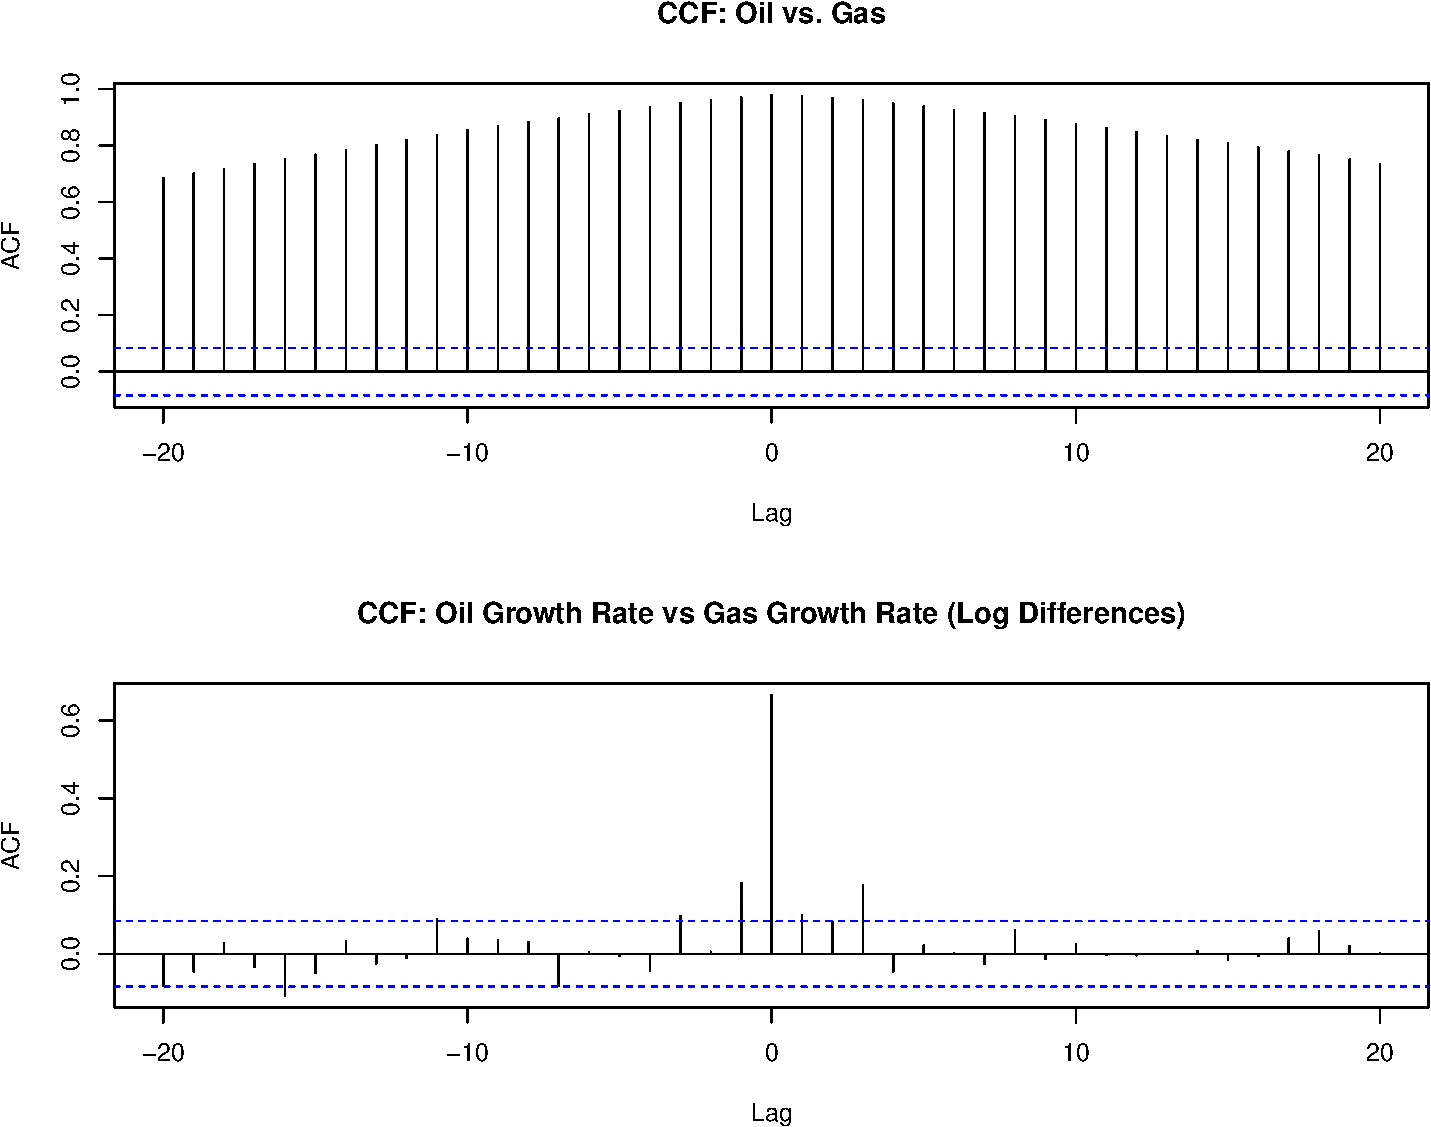
\includegraphics[width=\linewidth]{Homework3_files/figure-latex/unnamed-chunk-5-1} \end{center}

\begin{Shaded}
\begin{Highlighting}[]
\CommentTok{\# Extract key values.}
\NormalTok{raw\_max\_idx }\OtherTok{\textless{}{-}} \FunctionTok{which.max}\NormalTok{(}\FunctionTok{abs}\NormalTok{(cc\_raw}\SpecialCharTok{$}\NormalTok{acf))}
\NormalTok{tr\_max\_idx  }\OtherTok{\textless{}{-}} \FunctionTok{which.max}\NormalTok{(}\FunctionTok{abs}\NormalTok{(cc\_tr}\SpecialCharTok{$}\NormalTok{acf))}
\NormalTok{raw\_max\_lag }\OtherTok{\textless{}{-}} \FunctionTok{as.numeric}\NormalTok{(cc\_raw}\SpecialCharTok{$}\NormalTok{lag[raw\_max\_idx])}
\NormalTok{tr\_max\_lag  }\OtherTok{\textless{}{-}} \FunctionTok{as.numeric}\NormalTok{(cc\_tr}\SpecialCharTok{$}\NormalTok{lag[tr\_max\_idx])}
\end{Highlighting}
\end{Shaded}

For the original data, CCF is extremely high at many nearby lags (max absolute CCF \(=0.978\) at lag 0), which is typical for two trending/nonstationary series. For transformed growth rates, the dominant spike is at lag 0 (CCF \(=0.665\)). There are also nearby spikes at lag \(-1\) (about 0.182), lag \(-3\) (about 0.097), lag \(+1\) (about 0.100), and lag \(+3\) (about 0.177) albeit much lower spikes.

\newpage

\subsection{Problem 1 (d)}\label{problem-1-d}

\begin{problem}[Problem 1 (d)]
Based on the CCF relation, which regression model would you propose between transformed gas (\texttt{pgas}) and oil (\texttt{poil}) prices.
\end{problem}

Using common-sense economics, oil prices should lead gas prices, so for modeling current gas growth \(G_t\) we should prioritize contemporaneous and negative CCF lags (current or past oil), not positive lags (future oil). In the transformed CCF, lag 0 is strongest and lag \(-1\) is the strongest negative nonzero lag, so the proposed model is:
\[
G_t = \beta_0 + \beta_1 O_t + \beta_2 O_{t-1} + W_t,
\]
which also matches the equation in part (f).

\newpage

\subsection{Problem 1 (e)}\label{problem-1-e}

\begin{problem}[Problem 1 (e)]
Exhibit scatterplots of the \texttt{poil} and \texttt{pgas} growth series for up to three weeks of lead time of oil prices and comment on the results (is the relationship positive or negative; is it linear or non-linear? Are there any outliers?).
\end{problem}

\begin{Shaded}
\begin{Highlighting}[]
\CommentTok{\# Display scatter plots.}
\FunctionTok{lag2.plot}\NormalTok{(}
\NormalTok{  poil, pgas, }\DecValTok{3}\NormalTok{,}
  \AttributeTok{xname =} \StringTok{\textquotesingle{}Weekly Oil Growth Rate (Log Differences)\textquotesingle{}}\NormalTok{,}
  \AttributeTok{yname =} \StringTok{\textquotesingle{}Weekly Gas Growth Rate (Log Differences)\textquotesingle{}}
\NormalTok{)}
\end{Highlighting}
\end{Shaded}

\begin{center}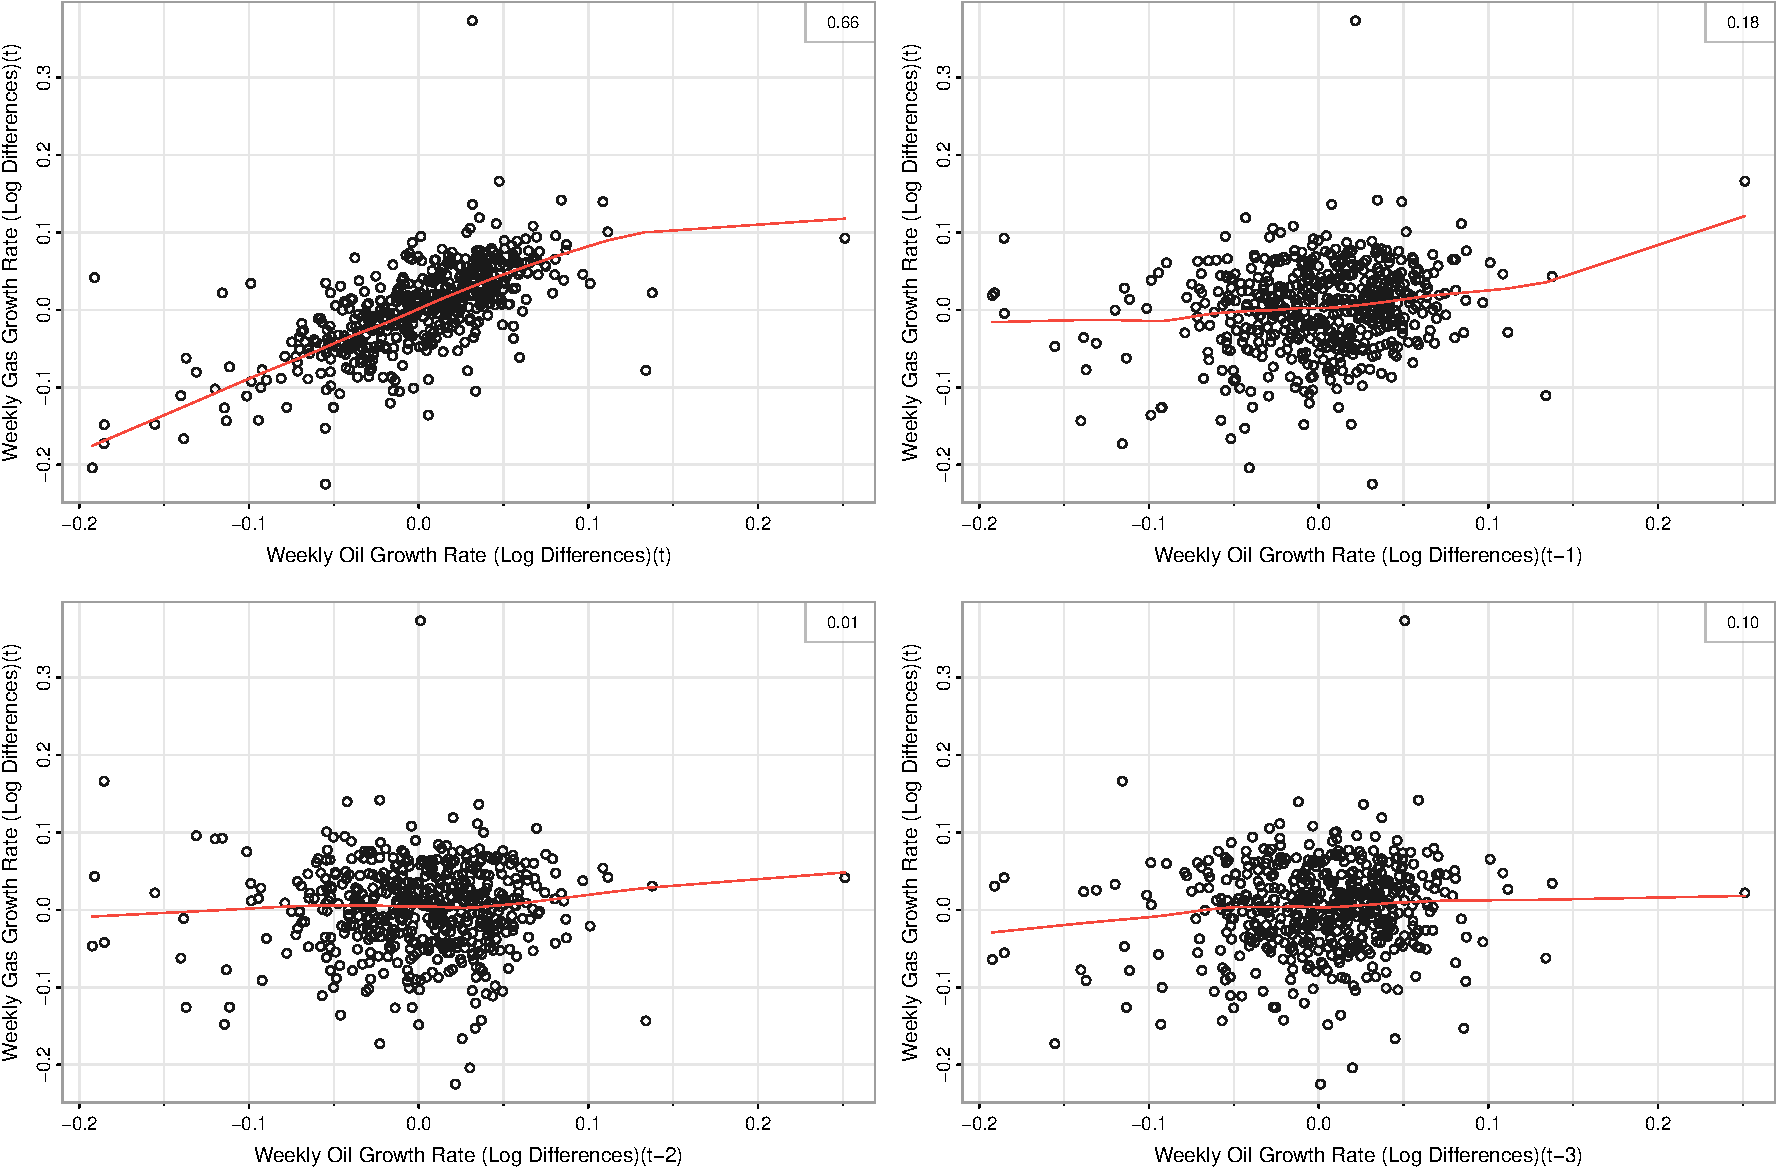
\includegraphics[width=\linewidth]{Homework3_files/figure-latex/unnamed-chunk-6-1} \end{center}

In the lead-0 panel (\(O_t\) versus \(G_t\)), the scatter plot shows a clear positive and roughly linear relationship, and this is the strongest association among the four panels. In the lead-1 panel (\(O_{t-1}\) versus \(G_t\)), the relationship is still positive but noticeably weaker, with a wider cloud around the trend. In the lead-2 panel (\(O_{t-2}\) versus \(G_t\)), the point cloud is much more diffuse and the linear pattern is weak to nearly absent. In the lead-3 panel (\(O_{t-3}\) versus \(G_t\)), a slight positive pattern reappears, but it is still weak relative to lead 0 and not as clean as lead 1. Across all panels, there are a few outlying points at the extremes (specifically, one that is very noticeable in all panels is the one with the relatively high weekly gas growth rate (log differences) compared to the rest).

\newpage

\subsection{Problem 1 (f)}\label{problem-1-f}

\begin{problem}[Problem 1 (f)]
Let \(G_t\) and \(O_t\) be the \texttt{pgas} and \texttt{poil} growth rates (transformed series) for gas at time \(t\) which varies from 2000 to 2010, then fit the following regression:
\[
G_t = \beta_0 + \beta_1 O_t + \beta_2 O_{t-1} + W_t
\]
Report the fitted model. Interpret the regression coefficients \(\beta_1\) and \(\beta_2\). Are the coefficients statistically significant. Is this a good model?
\end{problem}

\begin{Shaded}
\begin{Highlighting}[]
\CommentTok{\# Fit model.}
\NormalTok{mess\_f }\OtherTok{\textless{}{-}} \FunctionTok{ts.intersect}\NormalTok{(}
  \AttributeTok{G =}\NormalTok{ pgas,}
  \AttributeTok{O =}\NormalTok{ poil,}
  \AttributeTok{Olag1 =} \FunctionTok{lag}\NormalTok{(poil, }\SpecialCharTok{{-}}\DecValTok{1}\NormalTok{),}
  \AttributeTok{dframe =} \ConstantTok{TRUE}
\NormalTok{)}
\NormalTok{fit\_f }\OtherTok{\textless{}{-}} \FunctionTok{lm}\NormalTok{(G }\SpecialCharTok{\textasciitilde{}}\NormalTok{ O }\SpecialCharTok{+}\NormalTok{ Olag1, }\AttributeTok{data =}\NormalTok{ mess\_f)}

\CommentTok{\# Summarize model.}
\FunctionTok{summary}\NormalTok{(fit\_f)}
\end{Highlighting}
\end{Shaded}

\begin{verbatim}
## 
## Call:
## lm(formula = G ~ O + Olag1, data = mess_f)
## 
## Residuals:
##      Min       1Q   Median       3Q      Max 
## -0.18587 -0.02038 -0.00032  0.02059  0.34594 
## 
## Coefficients:
##              Estimate Std. Error t value             Pr(>|t|)    
## (Intercept) 0.0002036  0.0017984   0.113              0.90991    
## O           0.7816923  0.0385464  20.279 < 0.0000000000000002 ***
## Olag1       0.1159144  0.0386567   2.999              0.00284 ** 
## ---
## Signif. codes:  0 '***' 0.001 '**' 0.01 '*' 0.05 '.' 0.1 ' ' 1
## 
## Residual standard error: 0.04185 on 540 degrees of freedom
## Multiple R-squared:  0.4512, Adjusted R-squared:  0.4492 
## F-statistic:   222 on 2 and 540 DF,  p-value: < 0.00000000000000022
\end{verbatim}

Fitted model:
\[
\widehat G_t = 0.000204 + 0.781692 O_t + 0.115914 O_{t-1},
\]

where \(G_t\) and \(O_t\) are weekly log-growth rates (approximately weekly percent changes) from the 545-point weekly series over 2000 to mid-2010; after differencing and 1-week lag alignment, the fitted sample has \(n=543\) points.

\begin{itemize}
\tightlist
\item
  \(\hat{\beta}_1=0.782\) means a 1\% increase in oil weekly growth is associated with about 0.782\% increase in gas weekly growth in the same week (using log-change approximation), holding last week's oil growth rate constant.
\item
  \(\hat{\beta}_2=0.116\) means a 1\% increase in last week oil growth is associated with about 0.116\% increase in current gas growth, holding current week's oil growth rate constant.
\end{itemize}

\(O_t\) is highly significant (\(p < 2\times 10^{-16}\)) and \(O_{t-1}\) is significant (\(p = 0.002838\)), and the overall model is significant (F-test \(p < 2.2\times 10^{-16}\)). The coefficient of determination is \(R^2 = 0.451\), so the model explains about 45.1\% of the variation in weekly gas growth. The residual standard error is 0.0418 in log-growth units. This means on average, the predicted current gas growth rate is off from the actual current gas growth rate by about 0.0418 in transformed units. All in all, this is a decent model.

\newpage

\subsection{Problem 1 (g)}\label{problem-1-g}

\begin{problem}[Problem 1 (g)]
There have been a number of studies questioning whether gasoline prices respond more quickly when oil prices are rising than when oil prices are falling (“asymmetry”). We will attempt to explore this question with simple lagged regression model. Let \(G_t\) and \(O_t\) be the \texttt{pgas} and \texttt{poil} growth rates (transformed series) for gas at time \(t\) which varies from 2000 to 2010, then fit the following regression:
\[
G_t = \beta_0 + \beta_1 O_t + \beta_2 O_{t-1} + \beta_3 I_t + W_t
\]
Where \(I_t\) is an indicator which is 1 if \(O_t \ge 0\) and 0 otherwise, this is the indicator of no growth or positive growth in oil price. Report the fitted model. Interpret the regression coefficients \(\beta_1, \beta_2,\beta_3\). Are the coefficients statistically significant? Is this a good model?
\end{problem}

\begin{Shaded}
\begin{Highlighting}[]
\CommentTok{\# Fit model.}
\NormalTok{indi }\OtherTok{\textless{}{-}} \FunctionTok{ifelse}\NormalTok{(poil }\SpecialCharTok{\textless{}} \DecValTok{0}\NormalTok{, }\DecValTok{0}\NormalTok{, }\DecValTok{1}\NormalTok{)}
\NormalTok{mess\_g }\OtherTok{\textless{}{-}} \FunctionTok{ts.intersect}\NormalTok{(}
  \AttributeTok{G =}\NormalTok{ pgas,}
  \AttributeTok{O =}\NormalTok{ poil,}
  \AttributeTok{Olag1 =} \FunctionTok{lag}\NormalTok{(poil, }\SpecialCharTok{{-}}\DecValTok{1}\NormalTok{),}
  \AttributeTok{I =}\NormalTok{ indi,}
  \AttributeTok{dframe =} \ConstantTok{TRUE}
\NormalTok{)}
\NormalTok{fit\_g }\OtherTok{\textless{}{-}} \FunctionTok{lm}\NormalTok{(G }\SpecialCharTok{\textasciitilde{}}\NormalTok{ O }\SpecialCharTok{+}\NormalTok{ Olag1 }\SpecialCharTok{+}\NormalTok{ I, }\AttributeTok{data =}\NormalTok{ mess\_g)}

\CommentTok{\# Summarize model.}
\FunctionTok{summary}\NormalTok{(fit\_g)}
\end{Highlighting}
\end{Shaded}

\begin{verbatim}
## 
## Call:
## lm(formula = G ~ O + Olag1 + I, data = mess_g)
## 
## Residuals:
##      Min       1Q   Median       3Q      Max 
## -0.18451 -0.02161 -0.00038  0.02176  0.34342 
## 
## Coefficients:
##              Estimate Std. Error t value             Pr(>|t|)    
## (Intercept) -0.006445   0.003464  -1.860              0.06338 .  
## O            0.683127   0.058369  11.704 < 0.0000000000000002 ***
## Olag1        0.111927   0.038554   2.903              0.00385 ** 
## I            0.012368   0.005516   2.242              0.02534 *  
## ---
## Signif. codes:  0 '***' 0.001 '**' 0.01 '*' 0.05 '.' 0.1 ' ' 1
## 
## Residual standard error: 0.04169 on 539 degrees of freedom
## Multiple R-squared:  0.4563, Adjusted R-squared:  0.4532 
## F-statistic: 150.8 on 3 and 539 DF,  p-value: < 0.00000000000000022
\end{verbatim}

Fitted asymmetry model:
\[
\widehat G_t = -0.006445 + 0.683127 O_t + 0.111927 O_{t-1} + 0.012368 I_t,
\]
where \(I_t=1\) if \(O_t\ge 0\), and \(I_t=0\) otherwise. Here \(G_t\) and \(O_t\) are weekly log-growth rates (approximately weekly percent changes) from the 545-point weekly series over 2000 to mid-2010; after differencing and lag alignment with the indicator, the fitted sample has \(n=543\) points.

Partitioning by indicator gives two explicit cases:
\[
\text{Case 1 (nonnegative current oil growth): } I_t=1 \iff O_t\ge 0.
\]
\[
\widehat G_t \mid (I_t=1) = 0.005923 + 0.683127 O_t + 0.111927 O_{t-1},
\]
\[
\text{Case 2 (negative current oil growth): } I_t=0 \iff O_t<0.
\]
\[
\widehat G_t \mid (I_t=0) = -0.006445 + 0.683127 O_t + 0.111927 O_{t-1}.
\]

\begin{itemize}
\tightlist
\item
  \(\hat{\beta}_1=0.683\) means a 1\% increase in current oil growth is associated with about 0.683\% increase in current gas growth, holding last week's oil growth rate and the indicator term constant.
\item
  \(\hat{\beta}_2=0.112\) means a 1\% increase in last week oil growth is associated with about 0.112\% increase in current gas growth, holding current week's oil growth rate and the indicator term constant.
\item
  \(\hat{\beta}_3=0.012\) means when current oil growth is nonnegative (\(I_t=1\)), predicted gas growth is higher by about 0.0124 log-growth units than when current oil growth is negative (\(I_t=0\)), holding current and last week's oil growth rates constant.
\end{itemize}

\(O_t\) is highly significant (\(p < 2\times 10^{-16}\)), \(O_{t-1}\) is significant (\(p = 0.003846\)), and \(I_t\) is significant at the 5\% level (\(p = 0.02534\)). The coefficient of determination is \(R^2 = 0.456\), so the model explains about 45.6\% of the variation in weekly gas growth. The residual standard error is 0.0417 in log-growth units. This means on average, the predicted current gas growth rate is off from the actual current gas growth rate by about 0.0417 in transformed units. All in all, this is, again, a decent model, and since the indicator coefficient is statistically significant and positive, this model provides modest evidence of asymmetry.

\newpage

\section{Problem 2}\label{problem-2}

\begin{problem}[Problem 2]
For the average temperature data at New Haven (same as Homework 2), construct a model that accounts for seasonality using indicators as follows: regress average temperature on time (linear trend) and seasonal indicators.
\[
\textbf{Model 4: } AvgTemp_t = \beta_0 + \beta_1 t + \sum_{i=1}^{3}\gamma_i D_{i,t} + W_t
\]
Report the fitted model. Compare the fit of model 4 with models 1,2 and 3 from Homework 2 using \(R^2_{adj}\), AIC, AICc and BIC.
\end{problem}

\begin{Shaded}
\begin{Highlighting}[]
\CommentTok{\# Build New Haven average temperature quarterly ts (Jan, Apr, Jul, Oct).}
\NormalTok{nh }\OtherTok{\textless{}{-}} \FunctionTok{seasonal\_df}\NormalTok{(}\StringTok{\textquotesingle{}data/Climate\_Northeast\_NewHavenCT.xlsx\textquotesingle{}}\NormalTok{, }\DecValTok{1}\SpecialCharTok{:}\DecValTok{4}\NormalTok{)}
\NormalTok{AvgTemp }\OtherTok{\textless{}{-}} \FunctionTok{ts}\NormalTok{(nh}\SpecialCharTok{$}\NormalTok{Avg, }\AttributeTok{start =} \FunctionTok{c}\NormalTok{(}\FunctionTok{min}\NormalTok{(nh}\SpecialCharTok{$}\NormalTok{Year), }\DecValTok{1}\NormalTok{), }\AttributeTok{frequency =} \DecValTok{4}\NormalTok{)}

\CommentTok{\# Time + trigonometric regressors (models 1{-}3 from Homework 2).}
\NormalTok{t }\OtherTok{\textless{}{-}} \FunctionTok{time}\NormalTok{(AvgTemp)}
\NormalTok{s }\OtherTok{\textless{}{-}} \DecValTok{4}
\NormalTok{t2 }\OtherTok{\textless{}{-}}\NormalTok{ t}\SpecialCharTok{\^{}}\DecValTok{2} \SpecialCharTok{/} \FunctionTok{factorial}\NormalTok{(}\DecValTok{2}\NormalTok{)}
\NormalTok{cs1 }\OtherTok{\textless{}{-}} \FunctionTok{cos}\NormalTok{(}\DecValTok{2} \SpecialCharTok{*}\NormalTok{ pi }\SpecialCharTok{*}\NormalTok{ t }\SpecialCharTok{/}\NormalTok{ s)}
\NormalTok{sn1 }\OtherTok{\textless{}{-}} \FunctionTok{sin}\NormalTok{(}\DecValTok{2} \SpecialCharTok{*}\NormalTok{ pi }\SpecialCharTok{*}\NormalTok{ t }\SpecialCharTok{/}\NormalTok{ s)}
\NormalTok{cs2 }\OtherTok{\textless{}{-}} \FunctionTok{cos}\NormalTok{(}\DecValTok{4} \SpecialCharTok{*}\NormalTok{ pi }\SpecialCharTok{*}\NormalTok{ t }\SpecialCharTok{/}\NormalTok{ s)}
\NormalTok{sn2 }\OtherTok{\textless{}{-}} \FunctionTok{sin}\NormalTok{(}\DecValTok{4} \SpecialCharTok{*}\NormalTok{ pi }\SpecialCharTok{*}\NormalTok{ t }\SpecialCharTok{/}\NormalTok{ s)}
\NormalTok{m1 }\OtherTok{\textless{}{-}} \FunctionTok{lm}\NormalTok{(AvgTemp }\SpecialCharTok{\textasciitilde{}}\NormalTok{ t }\SpecialCharTok{+}\NormalTok{ cs1 }\SpecialCharTok{+}\NormalTok{ sn1)}
\NormalTok{m2 }\OtherTok{\textless{}{-}} \FunctionTok{lm}\NormalTok{(AvgTemp }\SpecialCharTok{\textasciitilde{}}\NormalTok{ t }\SpecialCharTok{+}\NormalTok{ t2 }\SpecialCharTok{+}\NormalTok{ cs1 }\SpecialCharTok{+}\NormalTok{ sn1)}
\NormalTok{m3 }\OtherTok{\textless{}{-}} \FunctionTok{lm}\NormalTok{(AvgTemp }\SpecialCharTok{\textasciitilde{}}\NormalTok{ t }\SpecialCharTok{+}\NormalTok{ t2 }\SpecialCharTok{+}\NormalTok{ cs1 }\SpecialCharTok{+}\NormalTok{ sn1 }\SpecialCharTok{+}\NormalTok{ cs2 }\SpecialCharTok{+}\NormalTok{ sn2)}

\CommentTok{\# Model 4: linear trend + seasonal indicators.}
\NormalTok{n }\OtherTok{\textless{}{-}} \FunctionTok{length}\NormalTok{(AvgTemp)}
\NormalTok{D1 }\OtherTok{\textless{}{-}} \FunctionTok{rep}\NormalTok{(}\DecValTok{0}\NormalTok{, n)  }\CommentTok{\# January}
\NormalTok{D2 }\OtherTok{\textless{}{-}} \FunctionTok{rep}\NormalTok{(}\DecValTok{0}\NormalTok{, n)  }\CommentTok{\# April}
\NormalTok{D3 }\OtherTok{\textless{}{-}} \FunctionTok{rep}\NormalTok{(}\DecValTok{0}\NormalTok{, n)  }\CommentTok{\# July}
\NormalTok{D4 }\OtherTok{\textless{}{-}} \FunctionTok{rep}\NormalTok{(}\DecValTok{0}\NormalTok{, n)  }\CommentTok{\# October (baseline)}
\NormalTok{D1[}\FunctionTok{seq}\NormalTok{(}\DecValTok{1}\NormalTok{, n, }\AttributeTok{by =} \DecValTok{4}\NormalTok{)] }\OtherTok{\textless{}{-}} \DecValTok{1}
\NormalTok{D2[}\FunctionTok{seq}\NormalTok{(}\DecValTok{2}\NormalTok{, n, }\AttributeTok{by =} \DecValTok{4}\NormalTok{)] }\OtherTok{\textless{}{-}} \DecValTok{1}
\NormalTok{D3[}\FunctionTok{seq}\NormalTok{(}\DecValTok{3}\NormalTok{, n, }\AttributeTok{by =} \DecValTok{4}\NormalTok{)] }\OtherTok{\textless{}{-}} \DecValTok{1}
\NormalTok{D4[}\FunctionTok{seq}\NormalTok{(}\DecValTok{4}\NormalTok{, n, }\AttributeTok{by =} \DecValTok{4}\NormalTok{)] }\OtherTok{\textless{}{-}} \DecValTok{1}
\NormalTok{m4 }\OtherTok{\textless{}{-}} \FunctionTok{lm}\NormalTok{(AvgTemp }\SpecialCharTok{\textasciitilde{}}\NormalTok{ t }\SpecialCharTok{+}\NormalTok{ D1 }\SpecialCharTok{+}\NormalTok{ D2 }\SpecialCharTok{+}\NormalTok{ D3)}
\FunctionTok{summary}\NormalTok{(m4)}
\end{Highlighting}
\end{Shaded}

\begin{verbatim}
## 
## Call:
## lm(formula = AvgTemp ~ t + D1 + D2 + D3)
## 
## Residuals:
##      Min       1Q   Median       3Q      Max 
## -24.1538  -1.8000   0.2001   2.3617  20.2155 
## 
## Coefficients:
##                 Estimate   Std. Error t value             Pr(>|t|)    
## (Intercept)  12.77833534  40.79079329   0.313               0.7543    
## t             0.00001093   0.02056915   0.001               0.9996    
## D1          -10.01537642   1.09163168  -9.175 < 0.0000000000000002 ***
## D2           -2.55384069   1.09157112  -2.340               0.0201 *  
## D3            6.35384889   1.09153478   5.821         0.0000000175 ***
## ---
## Signif. codes:  0 '***' 0.001 '**' 0.01 '*' 0.05 '.' 0.1 ' ' 1
## 
## Residual standard error: 6.223 on 255 degrees of freedom
## Multiple R-squared:  0.4752, Adjusted R-squared:  0.467 
## F-statistic: 57.72 on 4 and 255 DF,  p-value: < 0.00000000000000022
\end{verbatim}

\begin{Shaded}
\begin{Highlighting}[]
\CommentTok{\# Comparison table.}
\NormalTok{comp2 }\OtherTok{\textless{}{-}} \FunctionTok{rbind}\NormalTok{(}
  \StringTok{\textquotesingle{}Model 1 (HW2)\textquotesingle{}} \OtherTok{=} \FunctionTok{fit\_stats}\NormalTok{(m1),}
  \StringTok{\textquotesingle{}Model 2 (HW2)\textquotesingle{}} \OtherTok{=} \FunctionTok{fit\_stats}\NormalTok{(m2),}
  \StringTok{\textquotesingle{}Model 3 (HW2)\textquotesingle{}} \OtherTok{=} \FunctionTok{fit\_stats}\NormalTok{(m3),}
  \StringTok{\textquotesingle{}Model 4 (Indicators)\textquotesingle{}} \OtherTok{=} \FunctionTok{fit\_stats}\NormalTok{(m4)}
\NormalTok{)}
\FunctionTok{table\_latex}\NormalTok{(}\FunctionTok{data.frame}\NormalTok{(}\AttributeTok{Model =} \FunctionTok{rownames}\NormalTok{(comp2), comp2, }\AttributeTok{row.names =} \ConstantTok{NULL}\NormalTok{), }\AttributeTok{digits =} \DecValTok{4}\NormalTok{)}
\end{Highlighting}
\end{Shaded}

\begin{center}

\begin{tabular}{cccccc}
\toprule
Model & Parameters & R2\_adj & AIC & AICc & BIC\\
\midrule
Model 1 (HW2) & 4 & -0.0116 & 7.1579 & 5.3209 & 7.2264\\
Model 2 (HW2) & 5 & -0.0124 & 7.1624 & 5.3258 & 7.2446\\
Model 3 (HW2) & 7 & -0.0202 & 7.1777 & 5.3420 & 7.2872\\
Model 4 (Indicators) & 5 & 0.4670 & 6.5210 & 4.6844 & 6.6032\\
\bottomrule
\end{tabular}
\end{center}

Model 4 fitted equation:
\[
\widehat{AvgTemp}_t =
12.7783 + 0.0000109266\,t
- 10.0154 D_{1,t}
- 2.5538 D_{2,t}
+ 6.3538 D_{3,t}.
\]
Furtheremore, the fitted model can be written as four seasonal equations:
\[
\text{January (}D_{1,t}=1,\;D_{2,t}=D_{3,t}=0\text{):}\quad
\widehat{AvgTemp}_t = 2.763 + 0.0000109266\,t.
\]
\[
\text{April (}D_{2,t}=1,\;D_{1,t}=D_{3,t}=0\text{):}\quad
\widehat{AvgTemp}_t = 10.2245 + 0.0000109266\,t.
\]
\[
\text{July (}D_{3,t}=1,\;D_{1,t}=D_{2,t}=0\text{):}\quad
\widehat{AvgTemp}_t = 19.1322 + 0.0000109266\,t.
\]
\[
\text{October (}D_{1,t}=D_{2,t}=D_{3,t}=0\text{):}\quad
\widehat{AvgTemp}_t = 12.7783 + 0.0000109266\,t.
\]
Here \(AvgTemp_t\) is New Haven average temperature in degrees Celsius. The time variable \(t\) is a quarterly time index in years, with frequency 4 (Jan, Apr, Jul, Oct), from 1950 to 2014.75 (1950 Q1 through 2014 Q4, although we know this is inconsistent from the raw data), with \(n=260\). Model 4 has much larger \(R^2_{adj}\) (0.467) than Models 1-3 (which are all near 0 or negative), and Model 4 also has the smallest AIC, AICc, and BIC in the comparison table. Therefore, among Models 1-4, the indicator-seasonality Model 4 provides the best fit for this New Haven average temperature series.

\end{document}
